\chapter{Literature Review}

The following chapter explains the concept of a data stream (\ref{sec:data_stream}), discusses advantages and disadvantages of multi-core (\ref{sec:multicore}), gives an overview of previous work on Apache Storm (\ref{sec:apache_storm}), and discusses other effort of porting distributed systems to multi-core (\ref{sec:similar_efforts}).

\section{Data Stream}
\label{sec:data_stream}

Data stream can be defined as ``a real-time, continuous, ordered (implicitly by arrival time or explicitly by timestamp) sequence of items. It is impossible to control the order in which items arrive, nor is it feasible to locally store a stream in its entirety" \citep{golab2003issues}.

\subsection{Comparison to a Database Management System}

Historically, data has been stored into database management systems (DBMS) where it was later analysed the assumption being that there would be enough disk space to contain the data. This approach fits many purposes but recently applications started "feeling the need" to analyse rapidly changing data on-the-fly.

This has brought on an advent of data stream processing. Several stream-processing frameworks have emerged such as Apache Storm \citep{ApacheStorm}, Apache Spark \citep{ApacheSpark}, and Yahoo S4 \citep{YahooS4}. These frameworks, usually ran on a cluster, provide the user with abstractions which greatly simplify writing a real-time data stream processing application.

Whereas DBMSs excel at getting an exact answer to a query, data streams usually provide an approximate answer. The answer is approximate because it is usually correct only within a certain window of time, the query is simplified because it can only be ran in one pass, or because it is used with a sampling rate which does not include all events. A typical data stream analysis using windows and sampling is depicted in figure \ref{fig:stream}.

\subsection{Querying a Data Stream}

The assumption behind using a time window is that users of the real-time system are most likely interested in the most recent events. Sampling, on the other hand, is used to reduce the number of events used for a query \citep{Gaber:2005:MDS:1083784.1083789}.

\begin{figure}[!htb]
	\centering
	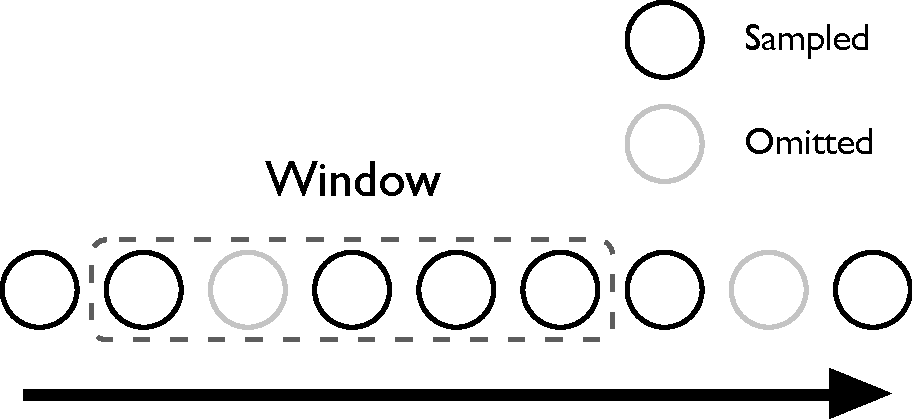
\includegraphics[scale=0.5]{pdf/stream.pdf}
	\caption{Stream Querying.}
	\label{fig:stream}
\end{figure}

Even though the answer might only be approximate it can have great value because the query is answered at the right time. Furthermore, even though the query may run only on a subset of data it is still possible to detect trends or system failures. For example, Twitter are using Apache Storm to run real-time analysis on millions of events per second for their analytics product \citep{Solovey}.

In research, several techniques have been developed to enable real-time data stream mining. For example, the MOA environment created by \citet{Bifet:2010:MMO:1756006.1859903} which enables real-time machine learning using the WEKA machine learning workbench \citep{Holmes1994}.

\section{Multi-core}
\label{sec:multicore}

A multi-core processor is a processor that has two or more independent execution cores. ``By providing multiple execution cores, each sequence of instructions, or thread, has a hardware execution environment entirely to itself. This enables each thread [to] run in a truly parallel manner" \citep{akhter2006multi}.

Running an application on multi-core can in the best case produce a speedup equivalent to the number of cores. The best case is when an application is embarrassingly parallel i.e. there is no inter-thread communication. Even though data stream processing is not an embarrassingly parallel problem, running a producer-consumer application on multiple cores can produce significant speedup \citep{Prat-Perez:2013:PPM:2450027.2450037} .

\subsection{Advantages Over Clusters}
\label{subsec:advantages}

There are several reasons why someone might prefer to deploy their data stream application to a single multi-core machine over a cluster:

\begin{description}
	\item[Communication Overhead] \hfill \\
	The latency of over-the-network communication is significantly higher than of two cores communicating on a single machine.
	\item[Lower Cost than a Data Centre] \hfill \\
	To run a distributed system on a cluster one would usually need to own a data centre. This comes with a high capital cost and increased maintenance costs than owning a single server.
	\item[More Control than with a Cloud Provider] \hfill \\
	Alternatively, one could rent out nodes on cloud computing services such as Amazon EC2 or Rackspace. While the cost of such services is acceptable the user does not have full control over their system.
\end{description}

\subsection{Disadvantages Over Clusters}
\label{subsec:disadvantages}

On the other hand, there are certain disadvantages in running a computation on a single multi-core machine rather than a cluster:

\begin{description}
	\item[Horizontal Scaling] \hfill \\
	Commodity hardware clusters offer better horizontal scaling than a single multicore server. If one needs to add nodes to the cluster it is as easy as purchasing more commodity hardware. On a multi-core machine it is not that simple. For example, a top of the line Intel\textsuperscript{\textregistered} Xeon\textsuperscript{\textregistered} Processor E5-2699 has support for 36 threads. Beyond that one would need to add another socket which essentially doubles the price. Moreover, the server would need to support multiple processor sockets.
	\item[Higher Short-term Cost than with a Cloud Provider] \hfill \\
	In short-term the cost of purchasing a server may be significantly higher than renting out a cluster from a cloud computing service. Thus, it makes most sense to run an application on multi-core if it is a long-term investment.
	\item[More Maintenance than with a Cloud Provider] \hfill \\
	Owning a server requires more maintenance than simply renting it out from a cloud provider. A cloud provider usually does  all the necessary maintenance and can provision a new machine very easily. Hence it is advantageous to use multi-core only if one can afford to maintain them as well.
\end{description}

It is generally believed that writing parallel software is hard. The traditional techniques of message passing and parallel threads sharing memory require the programmer to manage the concurrency at a fairly low level, either by using messages or locks.

Apache Storm has become the de facto tool used in stream processing on a cluster and according to their ``Powered By" page there are tens of companies already using Storm to process their real-time streams. It would be nice if they could keep that code.

\section{Apache Storm}
\label{sec:apache_storm}

Apache Storm is an open source distributed real-time computation system. Storm was Originally created by Nathan Marz while working at BackType. \cite{NathanAbout} BackType was later acquired by Twitter which is when Storm became open source. Storm was incubated into Apache with version 0.9.1 and became a top-level Apache project in September 2014.

Storm was developed to run on top of a cluster where nodes execute components of a computation in parallel. Running Storm on a cluster of commodity hardware gives it good horizontal scaling properties. Running separate components in parallel allows the system to execute in real time.

\subsection{Dependencies}

Storm has five major dependencies:

\begin{description}
	\item[Apache Zookeeper] \hfill \\
	Apache Zookeeper \citep{ApacheZookeeper} is an open source server that allows reliable distributed coordination. Storm uses Apache Zookeeper to maintain state which is then read and written to by nodes of a Storm cluster. More detail on how Storm uses Zookeeper is given in section \ref{subsec:zookeeper}.
	\item[Apache Thrift] \hfill \\
	Apache Thrift \citep{ApacheThrift} is a cross-language framework for developing services. It allows you to write a definition file for services and data types required by your application and automatically generates interface code which supports remote procedure calls and serialisation of the data types.
	\item[Kryo] \hfill \\
	Kryo \citep{EsotericKryo} is a serialisation library. It is used by Storm to serialise objects when sent over the network between nodes of a cluster.
	\item[Netty] \hfill \\
	Netty \citep{Netty} is an asynchronous event-driven network application framework. Storm utilises Netty to send intra-cluster messages. Thus when a node produces a result to be consumed by another node of the cluster it sends a message over the network using the TCP protocol implemented in Netty.
	\item[LMAX Disruptor] \hfill \\
	LMAX Disruptor \cite{LMAXDisruptor} is a high-performance data structure used to exchange data between concurrent threads. It uses a lock-free implementation of a ring buffer which components of a Storm program running on the same node a cluster use to exchange messages.
\end{description}

\subsection{Usage of Apache Storm}

Storm works well with sister Apache projects such as Apache Kafka \cite{ApacheKafka} and Apache HBase \cite{ApacheHBase}. Apache Kafka is a messaging broker that is often used as the missing link between producers and consumers of a cluster. Apache HBase is a big data-store that allows real-time random reads and writes modelled after Google's Bigtable project \cite{Chang:2008:BDS:1365815.1365816}.

Storm is reportedly used by 81 companies listed on their website \cite{https://storm.apache.org/documentation/Powered-By.html} and possibly many others. Storm's popularity is one of the reasons why it was chosen for this project. Moreover, we believe that the concepts used in Storm (explained further in section \ref{sec:concepts}) apply to many different situations and many applications can be easily adapter to work on Storm.

There has been research into how to optimise computations running on a Storm cluster. \cite{Chatzistergiou:2014:FHN:2661829.2661882} looked at how to reconfigure the job by reallocating component tasks to minimise communication cost. 

\section{Similar Efforts}
\label{sec:similar_efforts}

Currently data stream processing is a province of distributed systems such as the ones mentioned in the previous section. Most languages support parallel execution and there are many libraries that ease the process of writing parallel programs on a single multi-core machine. However, they are not tailored to data stream processing and usually require the programmer to do the heavy lifting rather than abstract it away.

There has been effort to port Hadoop to multi-core in \citep{Kumar:2013:HSD:2536274.2536314} (Hone) as well as port of Google's MapReduce in \citep{ranger2007evaluating} (Phoenix). However, to our knowledge there has not been effort to port Storm or any other real-time data stream framework to multi-core.

\section{Summary}

Distributed real-time computation systems such as Apache Storm provide programmers with abstractions that make it very easy to implement a data stream processing applications on top of  a cluster. However, in case of single multi-core machines there are not any obvious software choices. While several frameworks that allow the programmer to parallelise the computation exist, they are not really tailored to data stream processing.

The following chapters provide a closer analysis of Apache Storm as well as a port of Apache Storm for a single multi-core machine.
